\documentclass[a4paper,kulak]{kulakarticle} %options: kul or kulak (default)

\usepackage[dutch]{babel}
\usepackage{hyperref}
\usepackage{graphicx}
\usepackage{amsmath,amssymb,amsthm}
\usepackage{siunitx}
\usepackage{pdfpages}
\usepackage{subfig}

\date{Academiejaar 2020 -- 2021}
\address{
  Ingenieurswetenschappen\\
  Probleemoplossen en Ontwerpen deel 2 \\
  Kevin Truyaert, Benjamin Maveau en Martijn Boussé}
\title{Elektrische circuits}
\author{Groep 6}


\begin{document}

\maketitle
\\
\section*{elektrische circuits}
Dit zijn grafische modellen van de elektrische circuits die we nodig hebben om ons wagentje ineen te steken. 
\section{afstandssensor}
Dit is de visualisatie van het circuit tussen de afstandssensor en de microcontroller.
	\begin{figure}[h]
		\centering
		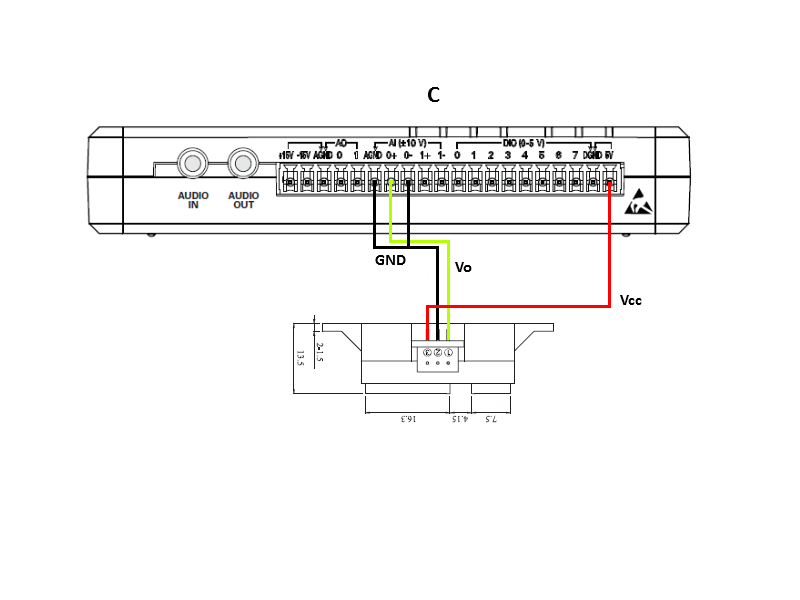
\includegraphics[width=.5\textwidth]{ECdistanceSensor} 
		\caption{elektrisch circuit afstandssensor}
		\label{fig:afstandssensor}
	\end{figure}

\section{reflectiesensor}
Dit is de visualisatie van het circuit tussen de reflectiesensor en de microcontroller.  
	\begin{figure}[h]
		\centering
		\includegraphics[width=.5\textwidth]{ECReflectionSensor } 
		\caption{elektrisch circuit reflectiesensor}
		\label{fig:reflectiesensor}
	\end{figure}
\section*{besluit}
Dit document toonde al onze elektrische circuits die we in de loop van dit vak zullen nodig hebben.  
\clearpage
\end{document}
